\section{Setup}

Both of our setups are identical wit the suggested in the exercise, with the exception of the insertion of a concave and a convex lens to ensure that the light-waves in the beam are parallel, and two mirror before the actual interferometer, to make adjustments of the beam easier. 

\subsection{Michelson Interferometer}

The piezo-electric material was driven by a frequency generator wich translated a vltage into a frequency. This apparatus is not showcased in the picture. 

\begin{figure}[H]
	\caption{Michelson Interferometer. 1. Helium laser 633 nm, 2. concave lense focal length $5$ cm, 3. Convex lense focal length $15$ cm, 4. mirror, 5. mirror, 6. beamsplitter, 7 piezo-electric material, 8. mirror, 9. detector}
	\centering
	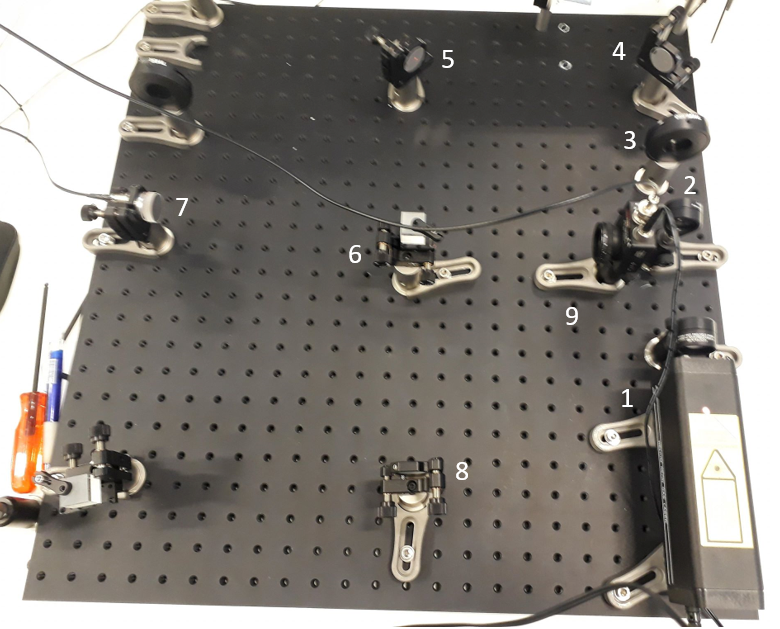
\includegraphics[width=0.5\textwidth]{Michelsonsetup}
\end{figure}

\subsection{Mach-Zender Interferometer}

\subsubsection{Refractive index}

The pressure in the glass tube were changed using a bike pump which is not visible on the picture. 


\begin{figure}[H]
	\caption{Mach-Zender interferometer used to measure refractive index. 1. Helium laser 633 nm, 2. concave lense focal length $5$ cm, 3. linear polarizer, 4. Convex lense focal length $15$ cm, 5. mirror, 6. mirror, 7. beamsplitter, 8. mirror, 9. mirror, 10. glass tube, 11. beamsplitter, 12. detector}
	\centering
	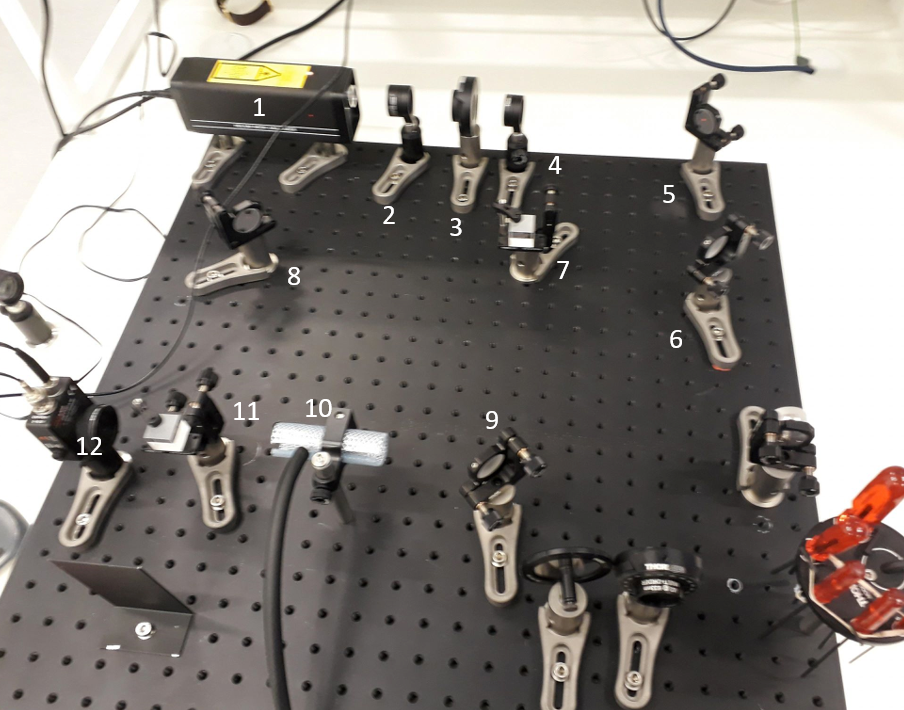
\includegraphics[width=0.5\textwidth]{MachZenderRI}
\end{figure}

\subsubsection{Lambda-half wheel}

\begin{figure}[H]
	\caption{Mach-Zender interferometer used to measure refractive index. 1. Helium laser 633 nm, 2. concave lense focal length $5$ cm and convex lense focal length $15$ cm, 3. mirror, 4. mirror, 5. beamsplitter, 6. $\frac{\lambda}{2}$-wheel,  7. mirror, 8. mirror, 9. beamsplitter, 10. detector}
	\centering
	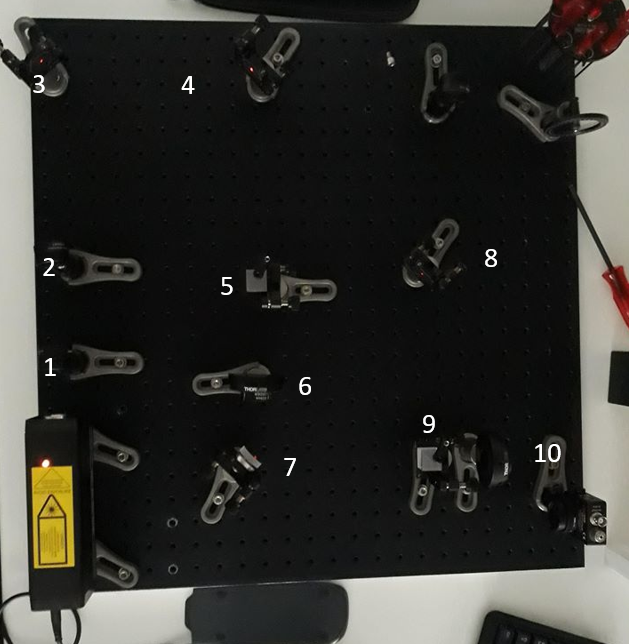
\includegraphics[width=0.5\textwidth]{MachZenderlambdahalv}
\end{figure}
